\documentclass{beamer}

\usetheme{CambridgeUS}
\usecolortheme{beaver}

\title{Fault Tolerance in Block-Level Caching}
\author{
  Jesus Ramos \and
  Douglas Otstott
}
\institute[FIU]{Florida International University}
\date{}

\begin{document}

\maketitle

\section{Problem Description}

\subsection{Problem Statement}

\begin{frame}
  \frametitle{Problem Statement}

  Fault tolerance in warehouse scale systems is an important issue
  \begin{itemize}
    \item Expect faults to happen
    \item Deal with faults online
  \end{itemize}

  Systems need to be
  \begin{itemize}
    \item Dependable and reliable
    \item Able to handle failure quickly and effectively
  \end{itemize}

\end{frame}

% end subsection Problem Statement

\subsection{Background}

\begin{frame}
  \frametitle{Problem Background}

  Warehouse Scale Computing Architectures utilize Storage Area
  Networks for persistent storage
  \begin{itemize}
    \item Increase reliability
    \item Easy to migrate VMs
    \item Storage Bandwidth  = \textcolor{red}{Performance Bottleneck}
  \end{itemize}

  Storage Area Networks use caches
  \begin{itemize}
    \item Leverages network storage
    \item Large performance increase
    \item \textcolor{red}{Reduced fault tolerance}
  \end{itemize}

\end{frame}

\begin{frame}
  \frametitle{Problem Background}
  \begin{center}
    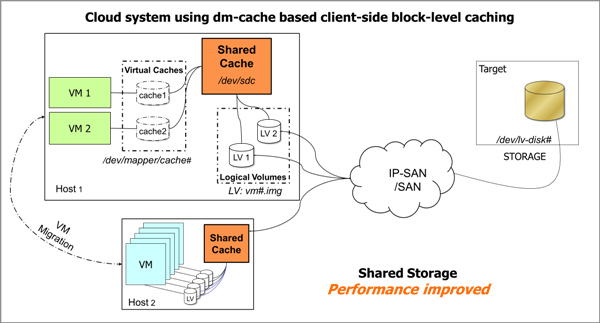
\includegraphics[scale=0.75]{../Images/NewerImage.png}
  \end{center}

  Cache device on host machine
  \begin{itemize}
    \item Virtual mapping between virtual disk and central storage
  \end{itemize}

\end{frame}

\begin{frame}
  \frametitle{DM-Cache}

  DM-Cache
  \begin{itemize}
    \item Open source block level (Linux Kernel module) caching
    solution
    \item Allows host machines to store recently used blocks
    \item Reduces the number of requests to central storage systems.
  \end{itemize}

  Increases performance
  \begin{itemize}
    \item Access time is much faster than central storage
    \item Greatly reduces contention for network storage
  \end{itemize}

  Decreases Fault Tolerance
  \begin{itemize}
    \item Metadata is non persistent
    \item Writes are buffered through the cache
    \item Local modifications are temporarily vulnerable
  \end{itemize}

\end{frame}

% end subsection Background

% end section Problem Description

\section{Proposed Solution}

\subsection{Metadata Persistence}

\begin{frame}
  \frametitle{Persist the Metadata}

  Solution
  \begin{itemize}
    \item Move the non-persistent metadata to the persistent cache
    device
    \begin{itemize}
      \item Facilitates the reconstruction of the cache
    \end{itemize}
    \item Cache the metadata in memory
    \begin{itemize}
      \item Write the data back asynchronously at certain intervals or
      every time it is updated
      \item Trade offs of write back methods
    \end{itemize}
  \end{itemize}

\end{frame}

% end subsection Metadata Persistence

% end section Proposed Solution

\section{Project Timeline}

\begin{frame}
  \frametitle{Tentative Timeline}
  \begin{description}
    \item[February 26th] - Begin Preliminary Testing (Radix Tree)
    \item[March 1st] - Begin solution implementation (Radix/Hash)
    \item[April 5th] - Debug solution (Hash Table)
    \item[April 10th] - Begin Evaluation
    \item[April 15th] - Conclude Evaluation
    \item[April 20th] - Write a paper and presentation
  \end{description}
\end{frame}

% end section Project Timeline

\section{Project Evaluation}

\begin{frame}
  \frametitle{Evaluation Criteria}

  In this project we will evaluate the following:
  \begin{itemize}
    \item The run-time overhead of two persistence techniques for
    metadata
    \begin{itemize}
      \item Updating the metadata in the background while keeping it
      cached on the disk
      \item Forcing a write back every time the metadata changes
    \end{itemize}
    \item The amount of time it takes to restore a cache to its last
    persistence point before the system failure
    \item The amount of data that can be recovered using both
    techniques
    \item The trade-offs between both techniques
    \begin{itemize}
      \item Data that can be recovered
      \item Run time overhead
    \end{itemize}
  \end{itemize}

\end{frame}

% end section Project Timeline

\section{Questions}

\begin{frame}
  \frametitle{Questions?}
\end{frame}

% end section Questions

\end{document}
